\chapter{实验结果与分析}

本章对SoCaffe的性能进行测试,首先给出GEMM加速器的独立测试结果,接着给出综合的SoCaffe性能测试。

GEMM测试主要包含GEMM设计过程中的各种优化策略的对比,并且从硬件资源使用和性能两个角度分析。此外,通过GEMM硬件版本与OpenBLAS的CPU版本的不同矩阵块尺寸下的对比,分析得到Caffe调用GEMM硬件操作的最佳时机。

综合SoCaffe测试分别测试了功能的完整性、计算速度与二者的综合。功能的完整性通过Caffe自带的单元测试进行分析;之后使用\texttt{convnet-benchmarks}\footnote{\url{https://github.com/pku-ceca-research/convnet-benchmarks}}作为基准进行卷积层的性能测试;最终,使用MNIST这一应用对SoCaffe进行整体评估。

\section{实验环境}

\begin{figure}[!ht]
	\centering	
	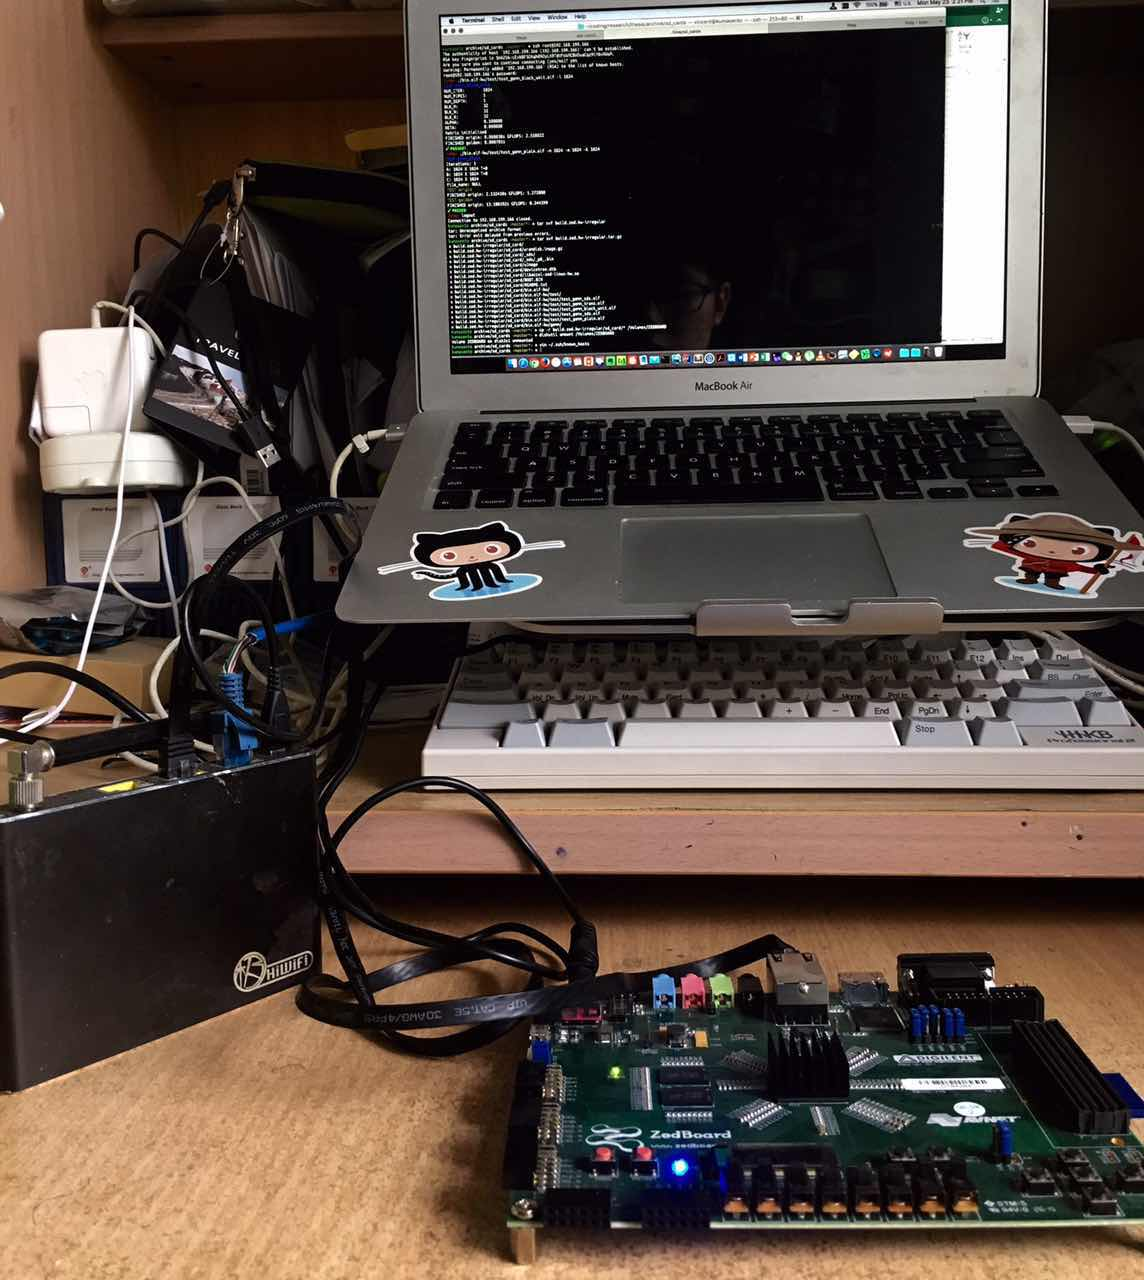
\includegraphics[width=0.6\textwidth]{assets/imgs/env.jpg}
	\caption{实验环境}
	\label{fig:env}
\end{figure}

本研究的实验环境如图\ref{fig:env}所示:Zedboard接上电源后与路由器LAN口通过以太网线连接,WAN口接入有线广域网,主机通过无线网络连接到路由器。配置路由器,令其分配给Zedboard一个固定的ip地址。之后主机即可通过ssh连接Zedboard进行测试。此外,所有的开发与编译过程都在ceca3主机完成,使用2015年4月推出的SDSoC开发平台。

\section{GEMM测试}

\subsection{优化策略对比}\label{subsec:compare}

根据\ref{subsec:gemmopt}节,以及加上\ref{subsubsec:normal},得到如下五个版本实现:原始实现(Baseline)、优化延迟(Latency)、资源分配优化(ResAlloc)、矩阵尺寸优化(IrrShape)以及半精度浮点数优化(HalfFloat)四个版本。本节选取四个版本的设计在最优参数配置下得到的实现作为对比样本,对比的项目包括:
\begin{enumerate}
\item 矩阵尺寸:根据目标版本,能得到的最优的矩阵尺寸;
\item FPGA资源利用:BRAM,DSP,LUT等指标所占用的百分比;
\item 延迟与时钟频率:时钟频率选用能综合得到的最快的时钟频率;
\item 预测性能与实际性能:用GFLOPS作为性能指标;
\end{enumerate}

% 实际性能测试
对实际性能的测试分为两种:GFLOPS块测试与完整测试:GFLOPS块测试只测试对一个GEMM固定矩阵块的计算时间,而GFLOPS完整测试的目标是\texttt{gemm\_sds}的时间,即测试任意大小矩阵的GEMM计算。

\begin{figure}[!ht]
	\centering	
	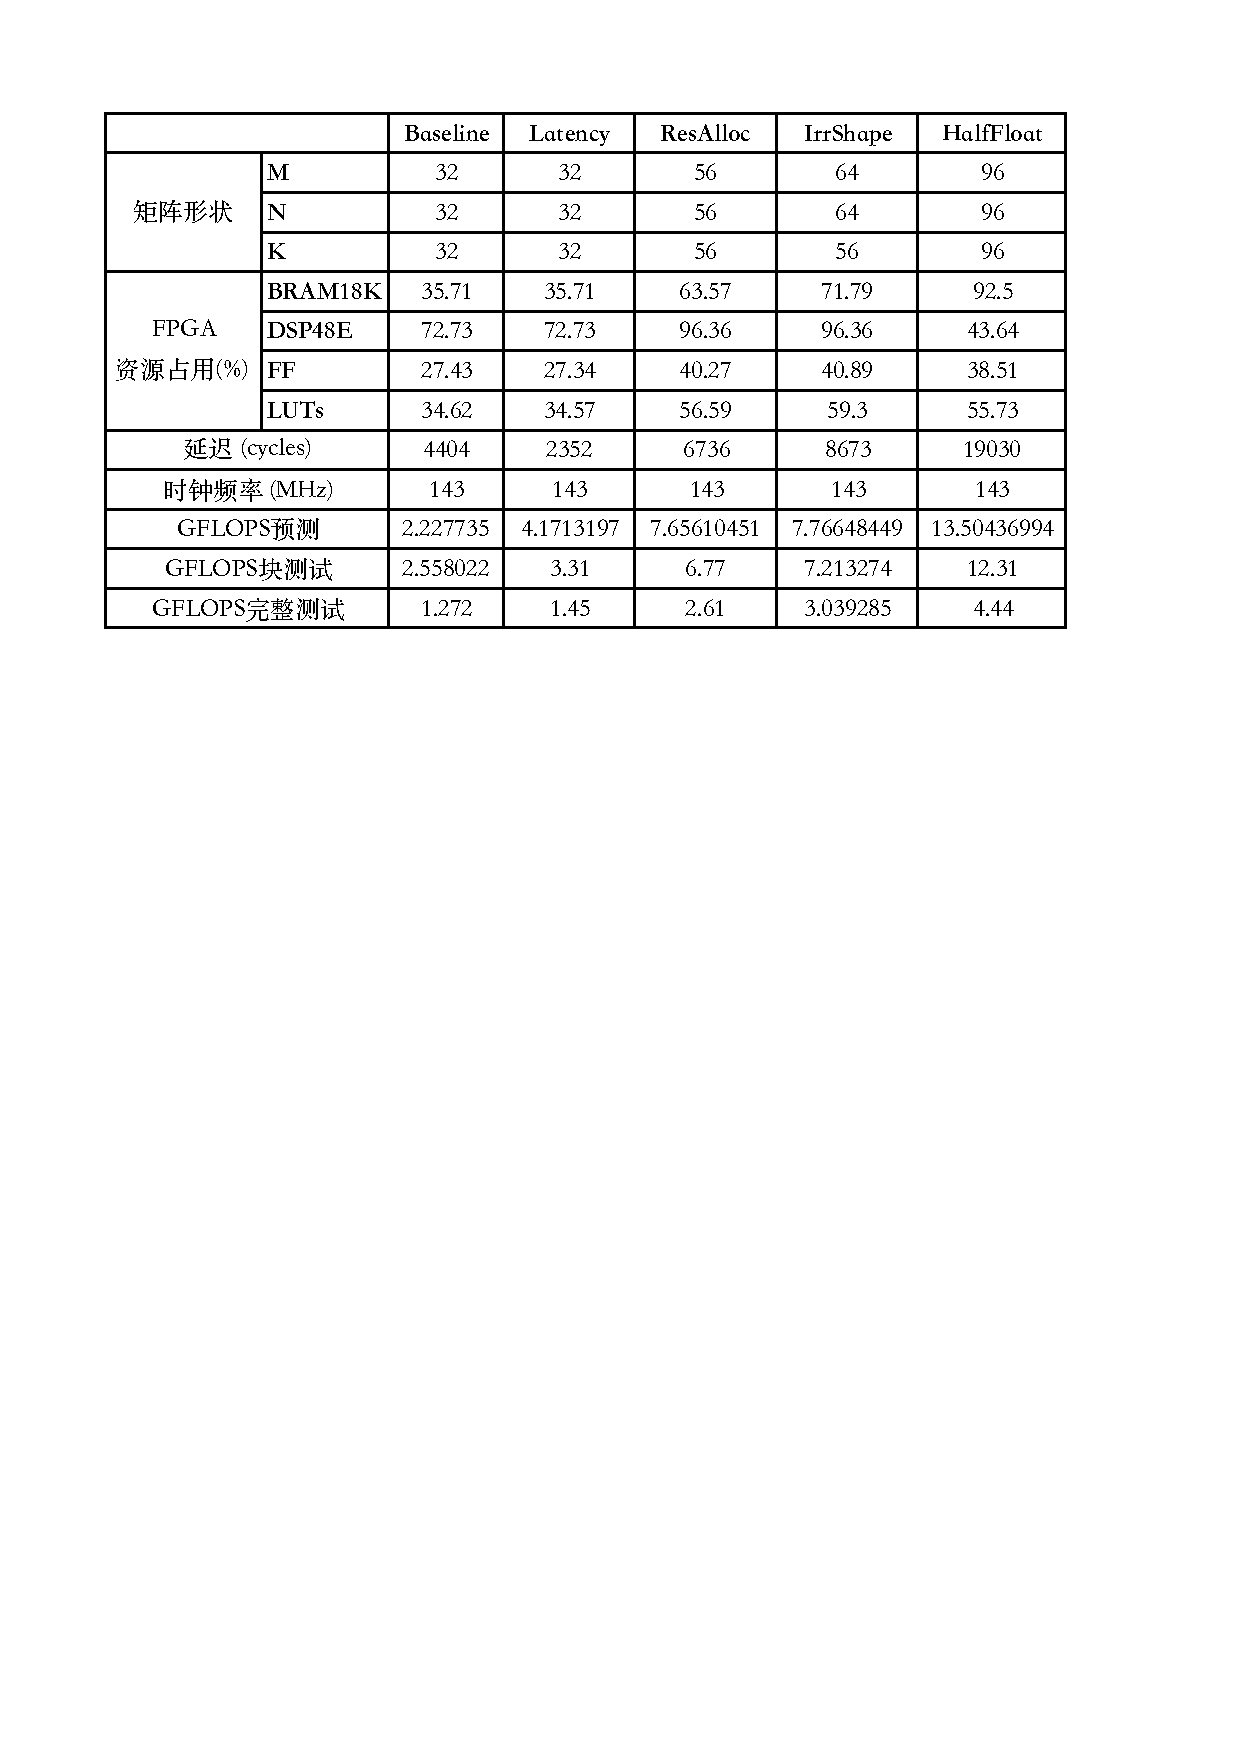
\includegraphics[width=\textwidth]{assets/imgs/gemmcomp.pdf}
	\caption{GEMM优化策略对比结果}
	\label{fig:gemmopt}
\end{figure}

对比结果参见图\ref{fig:gemmopt}。可以发现最快的优化版本是使用半精度浮点数优化的版本,GFLOPS与矩阵块的大小密切相关。尽管资源分配优化与矩阵尺寸优化在$K$对应的矩阵块尺寸上一致,但因为$M$与$N$的不同造成性能上矩阵尺寸优化略优。此外,发现GFLOPS完整测试的GFLOPS相比于块测试的GFLOPS要小,可以看出CPU端的计算确实比较影响最终的计算性能。

\subsection{OpenBLAS对比测试}

OpenBLAS是非常成熟的BLAS计算库,而且也是Caffe兼容的BLAS库之一,因此其在ARM CPU上的运行时间可以作为GEMM硬件加速比的计算基准。

\begin{figure}[!ht]
\centering	
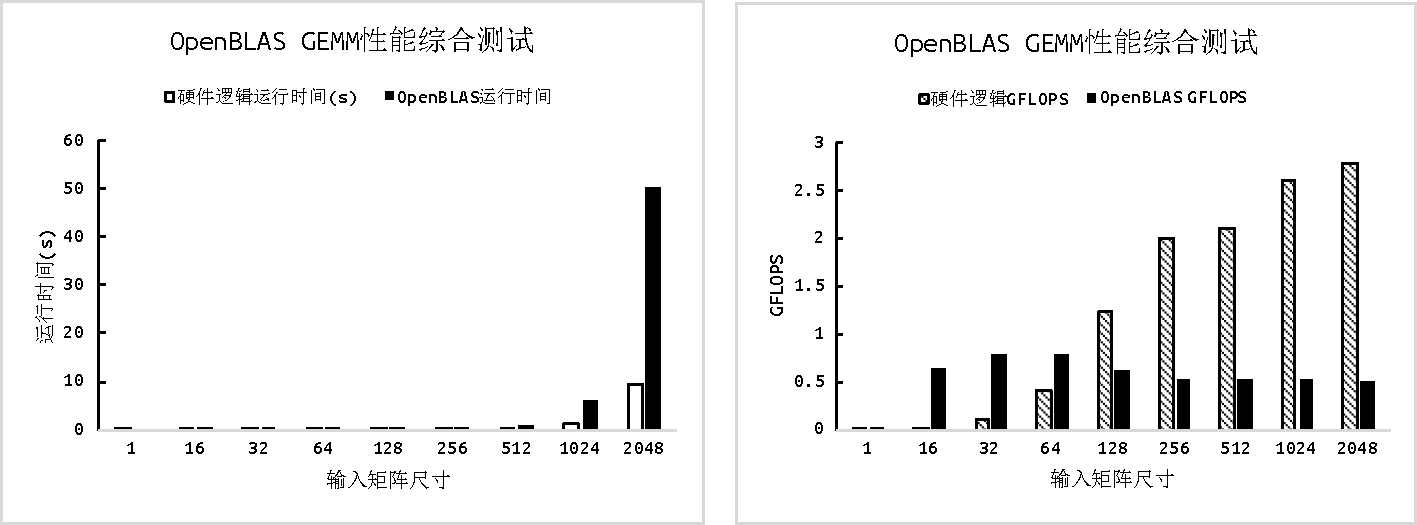
\includegraphics[width=\textwidth]{assets/imgs/gemmblas.pdf}
\caption{GEMM与OpenBLAS的性能对比}
\label{fig:gemmblas}
\end{figure}

这里测试使用的是GEMM在单精度浮点数精度下最快的版本(IrrShape)。与OpenBLAS在多种矩阵尺度下相比,GEMM硬件加速版本确实在小尺寸矩阵上速度很慢,但随着矩阵尺度大于128时,GEMM硬件加速比越来越大。最终测试结果显示GEMM的硬件加速版本是OpenBLAS的5.42倍。

此外,OpenBLAS对比测试与GEMM的完整测试都假定输入矩阵的尺寸一致。这种形式的输入对GEMM的分块计算很友好,很难出现划分不均匀的情况。但是实际中大部分矩阵形态都是不规则的,当划分矩阵块不均匀时,会造成额外的计算并降低性能。但是一般情况下,当矩阵尺寸本身比较大时,额外计算占比不多,对最终性能的影响也不十分显著。

\section{Caffe测试}

\subsection{单元测试}

Caffe的单元测试使用Google Test测试框架\footnote{Google Test\url{(https://github.com/google/googletest)}是一套基于C++的测试框架,提供完整的单元测试(xUnit)搭建功能。}进行搭建,在功能性测试的基础上也加上简单的对性能的测试。

经过运行Caffe的单元测试可以发现,几乎全部的测试都可以通过。但是对于少部分IO测试和HDF5的功能测试出现了问题。初步排查发现是Caffe的单元测试实现问题:部分数据文件在转换到ARM平台以后会无法读写。这类问题在使用lmdb的时候也出现过,需要重新生成一遍文件才能正常读取。由于大部分功能,尤其是关键的深度学习计算功能是完整的且没有问题的,因此本研究先将上述问题搁置,留待后续处理。

\subsection{卷积神经网络性能测试}

\begin{listing}[!ht]
\begin{minted}[
  mathescape, 
  linenos,
  numbersep=5pt,
  breaklines=true,
  fontsize=\footnotesize]{proto}
name: "ConvLayer_3x96x11x11"
input: "data"
input_dim: 32
input_dim: 3
input_dim: 32
input_dim: 32
force_backward: true
layers {
  name: "conv1"
  type: CONVOLUTION
  bottom: "data"
  top: "conv1"
  blobs_lr: 1
  blobs_lr: 2
  convolution_param {
    num_output: 96
    kernel_size: 11
    stride: 1
    weight_filler {
      type: "xavier"
    }
    bias_filler {
      type: "constant"
    }
  }
}
\end{minted}

\caption{卷积层性能测试Caffe网络文件}
\label{lst:convtest}
\end{listing}

由于本研究主要优化了卷积神经网络中需要用到的GEMM计算,因此这里对GEMM于Caffe的融合程度进行测试,观察Caffe的卷积层是否有不错的性能提升。

这里的测试用例使用的网络配置文件为\ref{lst:convtest},根据列举出的参数可以计算得传给GEMM的参数分别为$M=96$,$N=484$,$K=363$(forward计算,backword计算矩阵规模基本一致)。

使用\ref{subsec:compare}中出现的几个设计进行分别测试,基准是OpenBLAS实现的软件版本。测试数据使用Caffe的\texttt{time}指令得到,指定迭代次数为10次:
\begin{figure}[!ht]
	\centering	
	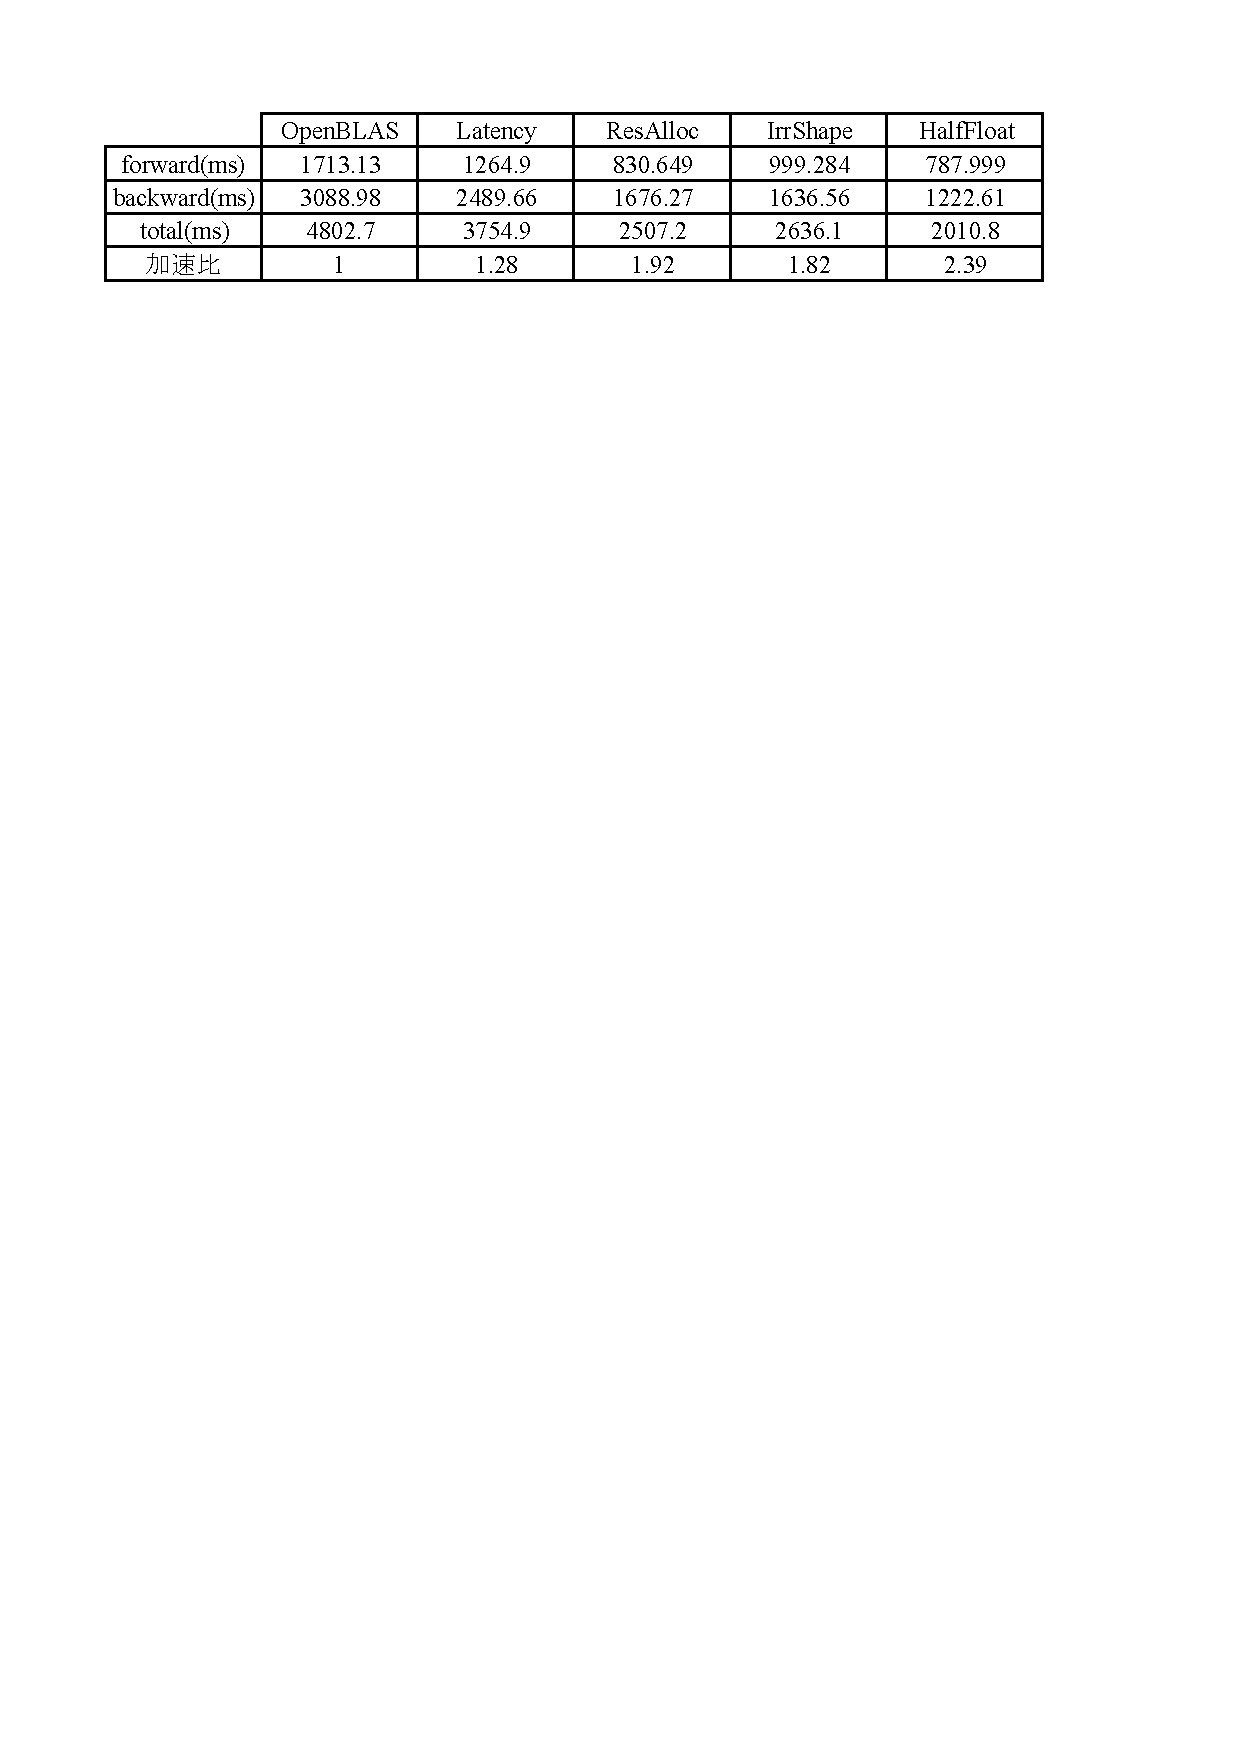
\includegraphics[width=\textwidth]{assets/imgs/caffeconv.pdf}
	\caption{Caffe的卷积层性能测试}
	\label{fig:caffeconv}
\end{figure}

表中的forward与backward分别为计算的前向与反向两个过程,根据结果可以发现最终加速比最高的来自于使用半精度浮点数的版本,达到2.39x。考虑到本测试用例使用的输入矩阵形状不规则,并且结合GEMM的独立测试的数据(\ref{fig:gemmopt}中半精度浮点数的完整测试GFLOPS为4.44),得到上述加速比基本合理。

\subsection{MNIST测试}

MNIST(Mixed National Institute of Standards and Technology)数据集包含大量手写字迹图片数据,常用作对机器学习算法的测试。LeNet\supercite{lecun1998gradient}是基于MNIST一种神经网络结构,因为它的网络结构比较小,并且包含了卷积层、池化层、全连接层和ReLU层,在网络层类型上也比较完整,所以本研究选用MNIST作为真实案例进行测试。

MNIST实现起来很简单,根据Caffe官方教程即可轻易搭建\footnote{\url{(http://caffe.berkeleyvision.org/gathered/examples/mnist.html)}}。由于在板上训练耗费内存较多,而且效率不高,因此训练过程在GPU主机完成,之后把训练结果复制到板上使用。

MNIST测试主要包含两个部分:性能测试与精度测试,性能测试使用\texttt{time}命令,精度测试使用\texttt{test}搭配之前的训练结果使用。得到的测试结果图\ref{fig:mnist}所示。

在\ref{fig:caffeconv}中表现优异的半精度浮点数的设计在MNIST网络中效率最低,主要是因为设置的96大小的矩阵块会在MNIST网络中造成过多的额外计算。表现最好的是Latency版本,但是与原始的OpenBLAS实现都相差不大。精度测试结果反映出所有的实现都拥有与标准实现一致的准确率,半精度浮点测试也如此,尽管半精度浮点数确实与单精度浮点数相比存在一定的误差。

总之,MNIST测试的结果主要反映出对于小规模的网络,加速比确实不够明显,而且并不是矩阵块越大效率越高:小规模的网络中额外计算占据的时间比更高。此外,半精度浮点数至少对于MNIST网络而言是完全没有准确率问题。其他网络在使用之前应先测试准确率。